\documentclass{standalone}
\usepackage{tikz}
\usetikzlibrary{patterns, positioning}


\begin{document}
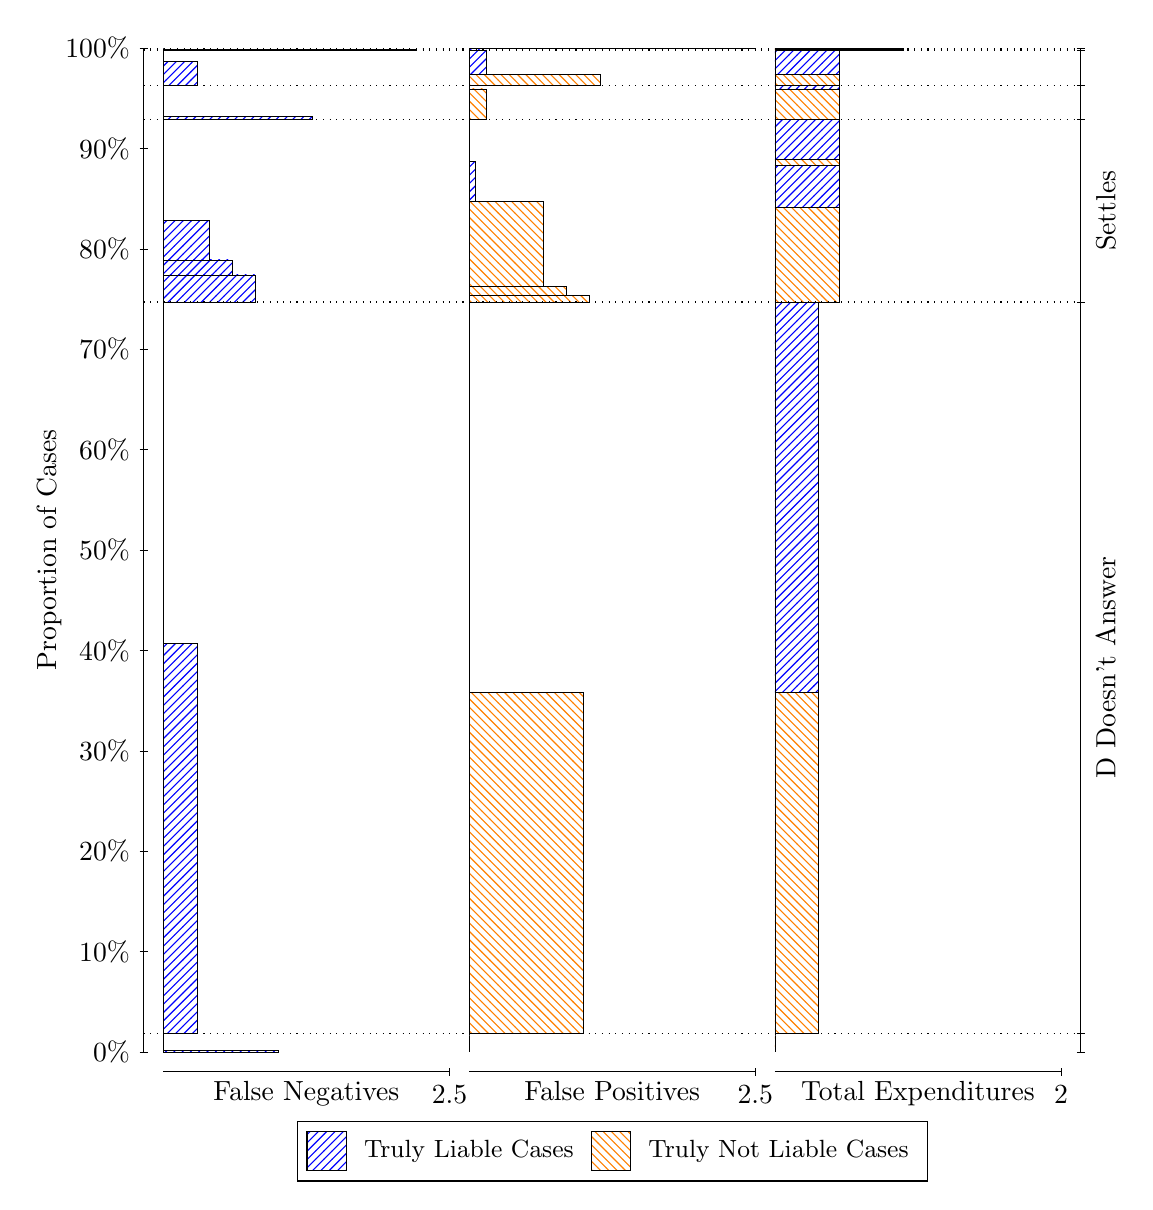
\begin{tikzpicture}
\draw[black, very thin] (1.5,1.75) -- (1.5,14.5);
\node[rotate=90, text=black, anchor=center] at (0.3, 8.125) {Proportion of Cases};
\draw[black, very thin] (1.45,1.75) -- (1.55,1.75);
\node[text=black, anchor=east] at (1.45, 1.75) {0\%};
\draw[black, very thin] (1.45,3.025) -- (1.55,3.025);
\node[text=black, anchor=east] at (1.45, 3.025) {10\%};
\draw[black, very thin] (1.45,4.3) -- (1.55,4.3);
\node[text=black, anchor=east] at (1.45, 4.3) {20\%};
\draw[black, very thin] (1.45,5.575) -- (1.55,5.575);
\node[text=black, anchor=east] at (1.45, 5.575) {30\%};
\draw[black, very thin] (1.45,6.85) -- (1.55,6.85);
\node[text=black, anchor=east] at (1.45, 6.85) {40\%};
\draw[black, very thin] (1.45,8.125) -- (1.55,8.125);
\node[text=black, anchor=east] at (1.45, 8.125) {50\%};
\draw[black, very thin] (1.45,9.4) -- (1.55,9.4);
\node[text=black, anchor=east] at (1.45, 9.4) {60\%};
\draw[black, very thin] (1.45,10.675) -- (1.55,10.675);
\node[text=black, anchor=east] at (1.45, 10.675) {70\%};
\draw[black, very thin] (1.45,11.95) -- (1.55,11.95);
\node[text=black, anchor=east] at (1.45, 11.95) {80\%};
\draw[black, very thin] (1.45,13.225) -- (1.55,13.225);
\node[text=black, anchor=east] at (1.45, 13.225) {90\%};
\draw[black, very thin] (1.45,14.5) -- (1.55,14.5);
\node[text=black, anchor=east] at (1.45, 14.5) {100\%};

\draw[black, very thin] (13.4,1.75) -- (13.4,14.5);
\draw[black, very thin] (13.35,1.75) -- (13.45,1.75);
\node[anchor=west] at (13.35, 1.75) {};
\draw[black, very thin] (13.35,1.9853) -- (13.45,1.9853);
\node[anchor=west] at (13.35, 1.9853) {};
\draw[black, very thin] (13.35,11.274) -- (13.45,11.274);
\node[anchor=west] at (13.35, 11.274) {};
\draw[black, very thin] (13.35,13.591) -- (13.45,13.591);
\node[anchor=west] at (13.35, 13.591) {};
\draw[black, very thin] (13.35,14.024) -- (13.45,14.024);
\node[anchor=west] at (13.35, 14.024) {};
\draw[black, very thin] (13.35,14.475) -- (13.45,14.475);
\node[anchor=west] at (13.35, 14.475) {};
\draw[black, very thin] (13.35,14.492) -- (13.45,14.492);
\node[anchor=west] at (13.35, 14.492) {};
\draw[black, very thin] (13.35,14.5) -- (13.45,14.5);
\node[anchor=west] at (13.35, 14.5) {};

\draw[black, very thin, pattern color=blue, pattern=north east lines] (1.75,1.75) rectangle (3.2033,1.7748);
\draw[black, very thin, pattern color=orange, pattern=north west lines] (1.75,1.7748) rectangle (1.75,1.9853);
\draw[black, very thin, pattern color=blue, pattern=north east lines] (1.75,1.9853) rectangle (2.186,6.9419);
\draw[black, very thin, pattern color=orange, pattern=north west lines] (1.75,6.9419) rectangle (1.75,11.274);
\draw[black, very thin, pattern color=blue, pattern=north east lines] (1.75,11.274) rectangle (2.9127,11.62);
\draw[black, very thin, pattern color=blue, pattern=north east lines] (1.75,11.62) rectangle (2.622,11.808);
\draw[black, very thin, pattern color=blue, pattern=north east lines] (1.75,11.808) rectangle (2.3313,12.311);
\draw[black, very thin, pattern color=orange, pattern=north west lines] (1.75,12.311) rectangle (1.75,13.591);
\draw[black, very thin, pattern color=blue, pattern=north east lines] (1.75,13.591) rectangle (3.6393,13.634);
\draw[black, very thin, pattern color=orange, pattern=north west lines] (1.75,13.634) rectangle (1.75,14.024);
\draw[black, very thin, pattern color=blue, pattern=north east lines] (1.75,14.024) rectangle (2.186,14.33);
\draw[black, very thin, pattern color=orange, pattern=north west lines] (1.75,14.33) rectangle (1.75,14.475);
\draw[black, very thin, pattern color=blue, pattern=north east lines] (1.75,14.475) rectangle (4.9473,14.48);
\draw[black, very thin, pattern color=orange, pattern=north west lines] (1.75,14.48) rectangle (1.75,14.492);
\draw[black, very thin, pattern color=orange, pattern=north west lines] (1.75,14.492) rectangle (1.75,14.496);
\draw[black, very thin, pattern color=blue, pattern=north east lines] (1.75,14.496) rectangle (1.75,14.5);
\draw[black, very thin, pattern color=orange, pattern=north west lines] (5.6333,1.75) rectangle (5.6333,1.9605);
\draw[black, very thin, pattern color=blue, pattern=north east lines] (5.6333,1.9605) rectangle (5.6333,1.9853);
\draw[black, very thin, pattern color=orange, pattern=north west lines] (5.6333,1.9853) rectangle (7.0867,6.3177);
\draw[black, very thin, pattern color=blue, pattern=north east lines] (5.6333,6.3177) rectangle (5.6333,11.274);
\draw[black, very thin, pattern color=orange, pattern=north west lines] (5.6333,11.274) rectangle (7.1593,11.354);
\draw[black, very thin, pattern color=orange, pattern=north west lines] (5.6333,11.354) rectangle (6.8687,11.476);
\draw[black, very thin, pattern color=orange, pattern=north west lines] (5.6333,11.476) rectangle (6.578,12.554);
\draw[black, very thin, pattern color=blue, pattern=north east lines] (5.6333,12.554) rectangle (5.706,13.058);
\draw[black, very thin, pattern color=blue, pattern=north east lines] (5.6333,13.058) rectangle (5.6333,13.591);
\draw[black, very thin, pattern color=orange, pattern=north west lines] (5.6333,13.591) rectangle (5.8513,13.981);
\draw[black, very thin, pattern color=blue, pattern=north east lines] (5.6333,13.981) rectangle (5.6333,14.024);
\draw[black, very thin, pattern color=orange, pattern=north west lines] (5.6333,14.024) rectangle (7.3047,14.17);
\draw[black, very thin, pattern color=blue, pattern=north east lines] (5.6333,14.17) rectangle (5.8513,14.475);
\draw[black, very thin, pattern color=orange, pattern=north west lines] (5.6333,14.475) rectangle (5.6333,14.488);
\draw[black, very thin, pattern color=blue, pattern=north east lines] (5.6333,14.488) rectangle (5.6333,14.492);
\draw[black, very thin, pattern color=orange, pattern=north west lines] (5.6333,14.492) rectangle (9.2667,14.496);
\draw[black, very thin, pattern color=blue, pattern=north east lines] (5.6333,14.496) rectangle (7.8133,14.5);
\draw[black, very thin, pattern color=orange, pattern=north west lines] (9.5167,1.75) rectangle (9.5167,1.9605);
\draw[black, very thin, pattern color=blue, pattern=north east lines] (9.5167,1.9605) rectangle (9.5167,1.9853);
\draw[black, very thin, pattern color=orange, pattern=north west lines] (9.5167,1.9853) rectangle (10.062,6.3177);
\draw[black, very thin, pattern color=blue, pattern=north east lines] (9.5167,6.3177) rectangle (10.062,11.274);
\draw[black, very thin, pattern color=orange, pattern=north west lines] (9.5167,11.274) rectangle (10.334,12.475);
\draw[black, very thin, pattern color=blue, pattern=north east lines] (9.5167,12.475) rectangle (10.334,13.008);
\draw[black, very thin, pattern color=orange, pattern=north west lines] (9.5167,13.008) rectangle (10.334,13.088);
\draw[black, very thin, pattern color=blue, pattern=north east lines] (9.5167,13.088) rectangle (10.334,13.591);
\draw[black, very thin, pattern color=orange, pattern=north west lines] (9.5167,13.591) rectangle (10.334,13.981);
\draw[black, very thin, pattern color=blue, pattern=north east lines] (9.5167,13.981) rectangle (10.334,14.024);
\draw[black, very thin, pattern color=orange, pattern=north west lines] (9.5167,14.024) rectangle (10.334,14.17);
\draw[black, very thin, pattern color=blue, pattern=north east lines] (9.5167,14.17) rectangle (10.334,14.475);
\draw[black, very thin, pattern color=orange, pattern=north west lines] (9.5167,14.475) rectangle (11.152,14.488);
\draw[black, very thin, pattern color=blue, pattern=north east lines] (9.5167,14.488) rectangle (11.152,14.492);
\draw[black, very thin, pattern color=orange, pattern=north west lines] (9.5167,14.492) rectangle (11.152,14.496);
\draw[black, very thin, pattern color=blue, pattern=north east lines] (9.5167,14.496) rectangle (11.152,14.5);
\draw[black, dotted] (1.5,1.9853) -- (13.4,1.9853);
\draw[black, dotted] (1.5,11.274) -- (13.4,11.274);
\draw[black, dotted] (1.5,13.591) -- (13.4,13.591);
\draw[black, dotted] (1.5,14.024) -- (13.4,14.024);
\draw[black, dotted] (1.5,14.475) -- (13.4,14.475);
\draw[black, dotted] (1.5,14.492) -- (13.4,14.492);
\draw[black, very thin] (1.75,1.5) -- (5.3833,1.5);
\node[text=black, anchor=north] at (3.5667, 1.5) {False Negatives};
\draw[black, very thin] (5.3833,1.45) -- (5.3833,1.55);
\node[text=black, anchor=north] at (5.3833, 1.45) {2.5};

\draw[black, very thin] (5.6333,1.5) -- (9.2667,1.5);
\node[text=black, anchor=north] at (7.45, 1.5) {False Positives};
\draw[black, very thin] (9.2667,1.45) -- (9.2667,1.55);
\node[text=black, anchor=north] at (9.2667, 1.45) {2.5};

\draw[black, very thin] (9.5167,1.5) -- (13.15,1.5);
\node[text=black, anchor=north] at (11.333, 1.5) {Total Expenditures};
\draw[black, very thin] (13.15,1.45) -- (13.15,1.55);
\node[text=black, anchor=north] at (13.15, 1.45) {2};


\node[text=black, centered, rotate=90] at (13.72, 6.6298) {D Doesn't Answer};
\node[text=black, centered, rotate=90] at (13.72, 12.433) {Settles};





\draw (7.449999999999999,1.5) node[draw=none] (baseCoordinate) {};
\begin{scope}[align=center]
        \matrix[scale=0.5, draw=black, below=0.5cm of baseCoordinate, nodes={draw}, column sep=0.1cm]{
            \node[rectangle, draw, minimum width=0.5cm, minimum height=0.5cm, pattern color=blue, pattern=north east lines] {}; &
            \node[draw=none, font=\small, text=black] (B) {Truly Liable Cases}; &
            \node[rectangle, draw, minimum width=0.5cm, minimum height=0.5cm, pattern color=orange, pattern=north west lines] {}; &
            \node[draw=none, font=\small, text=black] (B) {Truly Not Liable Cases}; \\
            };
\end{scope}

\end{tikzpicture}
\end{document}